\subsection{Model Organization}
The package diagram can be seen in figure \ref{fig:pkg} on page \pageref{fig:pkg}. As it can be seen in the figure, the top level is named PSOS( Particle Swarm Optimization System) note that the other packages connect to this namespace.
\\\\
A brief description of the content:
\begin{itemize}
	\item \nameref{requirementspecification:operation} contains Use Cases and Requirements diagrams, see page \pageref{requirementspecification:operation}.
	\item \nameref{requirementspecification:Structure} contains Block Definition and Internal Block diagrams, see page \pageref{requirementspecification:Structure}.
	\item \nameref{requirementspecification:Behavior} contains Activity, Sequence and State Machine diagrams, see page \pageref{requirementspecification:Behavior}.

\end{itemize}

\begin{figure}[H]
	\centering
	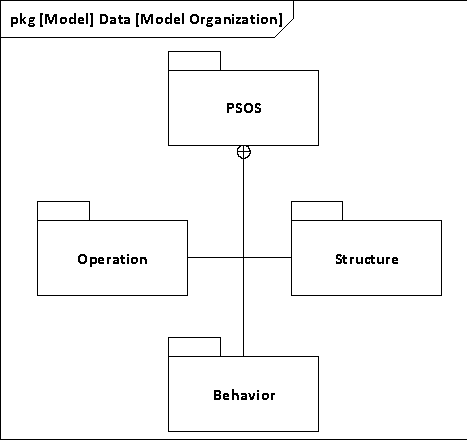
\includegraphics[width=0.7\linewidth]{diagram/pkg_data_model_organization.pdf}
	\caption{Package Diagram with the namespace PSOS}
	\label{fig:pkg}
\end{figure}